%======================================================================
% OPTION A — pgfplots scatter figure
%======================================================================

\begin{figure}[t]
    \centering
    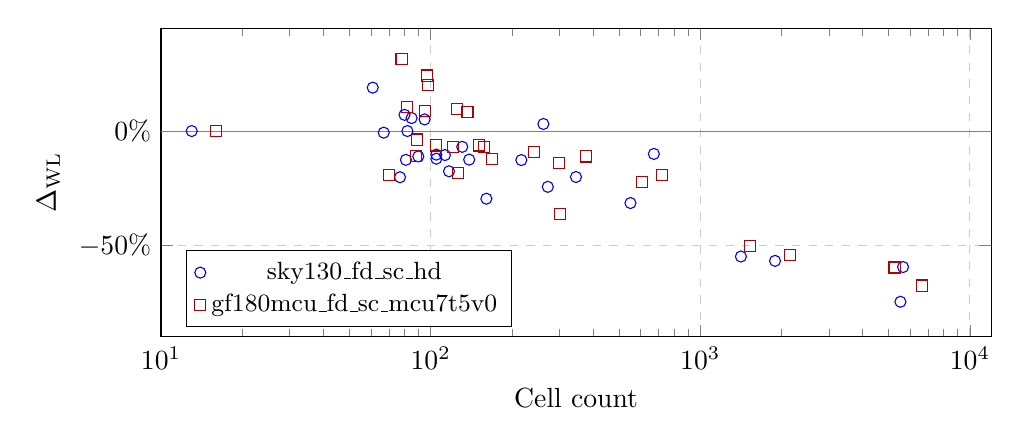
\begin{tikzpicture}
        \begin{semilogxaxis}[
            width=\columnwidth, height=5.5cm,
            xlabel={Cell count},
            ylabel={$\Delta_{\mathrm{WL}}$},
            ylabel style={align=center},
            xmin=10, xmax=12000,
            ymin=-90, ymax=45,
            yticklabel={\pgfmathprintnumber{\tick}\%},
            grid=major, grid style={dashed,gray!40},
            legend pos=south west,
            legend style={font=\small},
            mark size=2pt,
            clip=false,
            ]
            % zero line
            \draw[gray,thin] (axis cs:10,0) -- (axis cs:12000,0);

            \addplot[only marks, mark=o, blue] coordinates {
            (13,0.0)  % s27
            (61,19.0)  % s298
            (67,-0.7)  % s386
            (77,-20.2)  % s420
            (80,7.1)  % s349
            (81,-12.6)  % s382
            (82,-0.0)  % s344
            (85,5.7)  % s444
            (90,-11.1)  % s400
            (95,5.1)  % s526
            (105,-12.1)  % s641
            (105,-10.3)  % s713
            (113,-10.5)  % s1196
            (117,-17.6)  % s510
            (131,-6.9)  % s820
            (139,-12.5)  % s832
            (161,-29.6)  % s838
            (217,-12.7)  % s953
            (262,3.1)  % s1196b
            (272,-24.4)  % s1238
            (346,-20.1)  % s1423
            (551,-31.5)  % s9234
            (673,-10.0)  % s5378
            (1415,-54.9)  % s13207
            (1894,-56.8)  % s15850
            (5526,-74.7)  % s38584
            (5651,-59.5)  % s35932
            };
            \addlegendentry{sky130\_fd\_sc\_hd}
            \addplot[only marks, mark=square, red!70!black] coordinates {
            (16,0.0)  % s27
            (70,-19.2)  % s298
            (78,31.4)  % s386
            (82,10.6)  % s420
            (88,-10.9)  % s349
            (89,-3.7)  % s344
            (95,8.7)  % s382
            (97,24.3)  % s400
            (98,20.0)  % s444
            (105,-6.3)  % s526
            (121,-6.9)  % s1196
            (125,9.6)  % s641
            (126,-18.2)  % s713
            (137,8.2)  % s510
            (151,-6.3)  % s820
            (158,-6.9)  % s832
            (169,-12.3)  % s838
            (241,-9.3)  % s953
            (300,-13.8)  % s1196b
            (301,-36.3)  % s1238
            (378,-11.1)  % s1423
            (606,-22.2)  % s9234
            (719,-19.2)  % s5378
            (1529,-50.4)  % s13207
            (2158,-54.4)  % s15850
            (5255,-59.7)  % s35932
            (6650,-67.6)  % s38584
            };
            \addlegendentry{gf180mcu\_fd\_sc\_mcu7t5v0}
        \end{semilogxaxis}
    \end{tikzpicture}
    \caption{Per-design scan-chain routed wirelength improvement of \textsc{ScanOpt}
    (\emph{opt}) vs.\ placement-aware baseline (\emph{basic}) as a function of
    cell count. Negative values indicate improvement.}
    \label{fig:scanopt_scatter}
\end{figure}
